\documentclass[12pt]{article}

\usepackage{amsmath, amssymb, mathrsfs, fancyhdr}
\usepackage{syntonly, lastpage, hyperref, enumitem, graphicx}
\usepackage{biblatex}
\usepackage{booktabs}
\usepackage{float}

\addbibresource{references.bib}

\hypersetup{colorlinks = true, urlcolor = black}

\headheight     15pt
\topmargin      -1.5cm   % read Lamport p.163
\oddsidemargin  -0.04cm  % read Lamport p.163
\evensidemargin -0.04cm  % same as oddsidemargin but for left-hand pages
\textwidth      16.59cm
\textheight     23.94cm
\parskip         7.2pt   % sets spacing between paragraphs
\parindent         0pt   % sets leading space for paragraphs
\pagestyle{empty}        % Uncomment if don't want page numbers
\pagestyle{fancyplain}

\newcommand{\MAP}{{\text{MAP}}}
\newcommand{\argmax}{{\text{argmax}}}
\newcommand{\argmin}{{\text{argmin}}}
\newcommand{\Cov}{{\text{Cov}}}
\newcommand{\Var}{{\text{Var}}}
\newcommand{\logistic}{{\text{logistic}}}

\renewcommand{\arraystretch}{1.2}

\begin{document}

\lhead{Caleb Leedy}
\chead{Non-monotone Missingness}
%\chead{STAT 615 - Advanced Bayesian Methods}
%\rhead{Page \thepage\ of \pageref{LastPage}}
\rhead{\today}

\section*{The Problem with the Weighted Linear Model}

Besides the semiparametric model, we have been comparing our results to an 
optimal weighted linear model. This model can be summarized as the following:

\begin{itemize}
  \item[1.] For each segment $A_k$ with a distinct missing pattern, let 
    $G_k(Z)$ be the observed data in segment $A_k$.
  \item[2.] For each $A_k$, estimate $\theta = E[g(X, Y_1, Y_2)]$ as 
    $\hat \theta_k = E[g \mid G_k(Z)]$.
  \item[3.] Combine these estimates using the inverse variance weighted average
    of each $\hat \theta_k$:

    \[\hat \theta = \sum_{k} w_k \hat \theta_k \text{ where } 
      w_k = \frac{V(\hat \theta_k)}{\sum_k V(\hat \theta_k)}.\]
\end{itemize}

By linear model theory this is the BLUE in the linear model case, and
this works really well in Simulation 1 in which 

\begin{align*}
  \begin{bmatrix} x_i \\ e_{1i} \\ e_{1i} \end{bmatrix} 
  &\stackrel{ind}{\sim} N\left(
  \begin{bmatrix} 0 \\ 0 \\ 0 \end{bmatrix},
  \begin{bmatrix} 1 & 0 & 0 \\ 0 & 1 & \rho \\ 0 & \rho & 1 \end{bmatrix}
  \right)\\
  y_{1i} &= x_i + e_{1i} \\
  y_{2i} &= \theta + x_i + e_{2i} \\
  g(X, Y_1, Y_2) &= Y_2
\end{align*}

As demonstrated in Table~\ref{tab:sim1}, the WLS estimator outperforms all of 
the other estimators except the Oraclex estimator which uses all of the data 
and even some elements that are missing!

\begin{table}[ht!]
  \caption{True Theta is 5. $\Cov(e_1, e_2) = 0.5$}
  \label{tab:sim1}
  \centering
  \begin{tabular}[t]{lrrrr}
    \toprule
    Algorithm & Bias & SD & T-stat & P-val\\
    \midrule
    Oracle & 0.001 & 0.044 & 1.546 & 0.061\\
    Oraclex & 0.000 & 0.032 & 0.479 & 0.316\\
    CC & 0.002 & 0.058 & 1.549 & 0.061\\
    IPW & 0.006 & 0.210 & 1.504 & 0.066\\
    WLS & 0.001 & 0.040 & 1.207 & 0.114\\
    Prop & 0.002 & 0.051 & 1.911 & 0.028\\
    OptSemi & 0.002 & 0.051 & 1.964 & 0.025\\
    \bottomrule
  \end{tabular}
\end{table}

However, in Simulation 2, in which we keep the same setup as Simulation 1,
but change $g(X, Y_1, Y_2) = Y_1^2 Y_2$. In this case, we have 


\begin{table}[ht!]
  \caption{True g is 10. $\Cov(e_1, e_2) = 0.5$}
  \label{tab:sim2}
  \centering
  \begin{tabular}[t]{lrrrr}
    \toprule
    Algorithm & Bias & SD & T-stat & P-val\\
    \midrule
    Oracle & 0.007 & 0.529 & 0.741 & 0.229\\
    Oraclex & 0.004 & 0.475 & 0.510 & 0.305\\
    CC & 0.023 & 0.824 & 1.518 & 0.065\\
    IPW & 0.031 & 0.915 & 1.846 & 0.032\\
    WLS & -0.131 & 0.387 & -18.504 & 0.000\\
    Prop & 0.011 & 0.635 & 0.912 & 0.181\\
    SemiOpt & 0.011 & 0.636 & 0.983 & 0.163\\
    \bottomrule
  \end{tabular}
\end{table}

Table~\ref{tab:sim2} clearly shows that the WLS estimator is biased, but 
since this is a weighted average of unbiased linear estimators, how 
can this be biased?

The answer comes from the fact that we weight based on the variance of 
each unbiased estimator. A closer examination of how the bias of 
one of the estimators from $A_k$ affects variance can be seen in
Figure~\ref{fig:biasvar}.

\begin{figure}[ht!]
  \caption{A scatterplot of the Bias-Variance relationship for Section $A_{11}$,
  in which all of the data is observed. A similar relationship is found in each 
  of the other sections too.}
  \label{fig:biasvar}
  \centering
  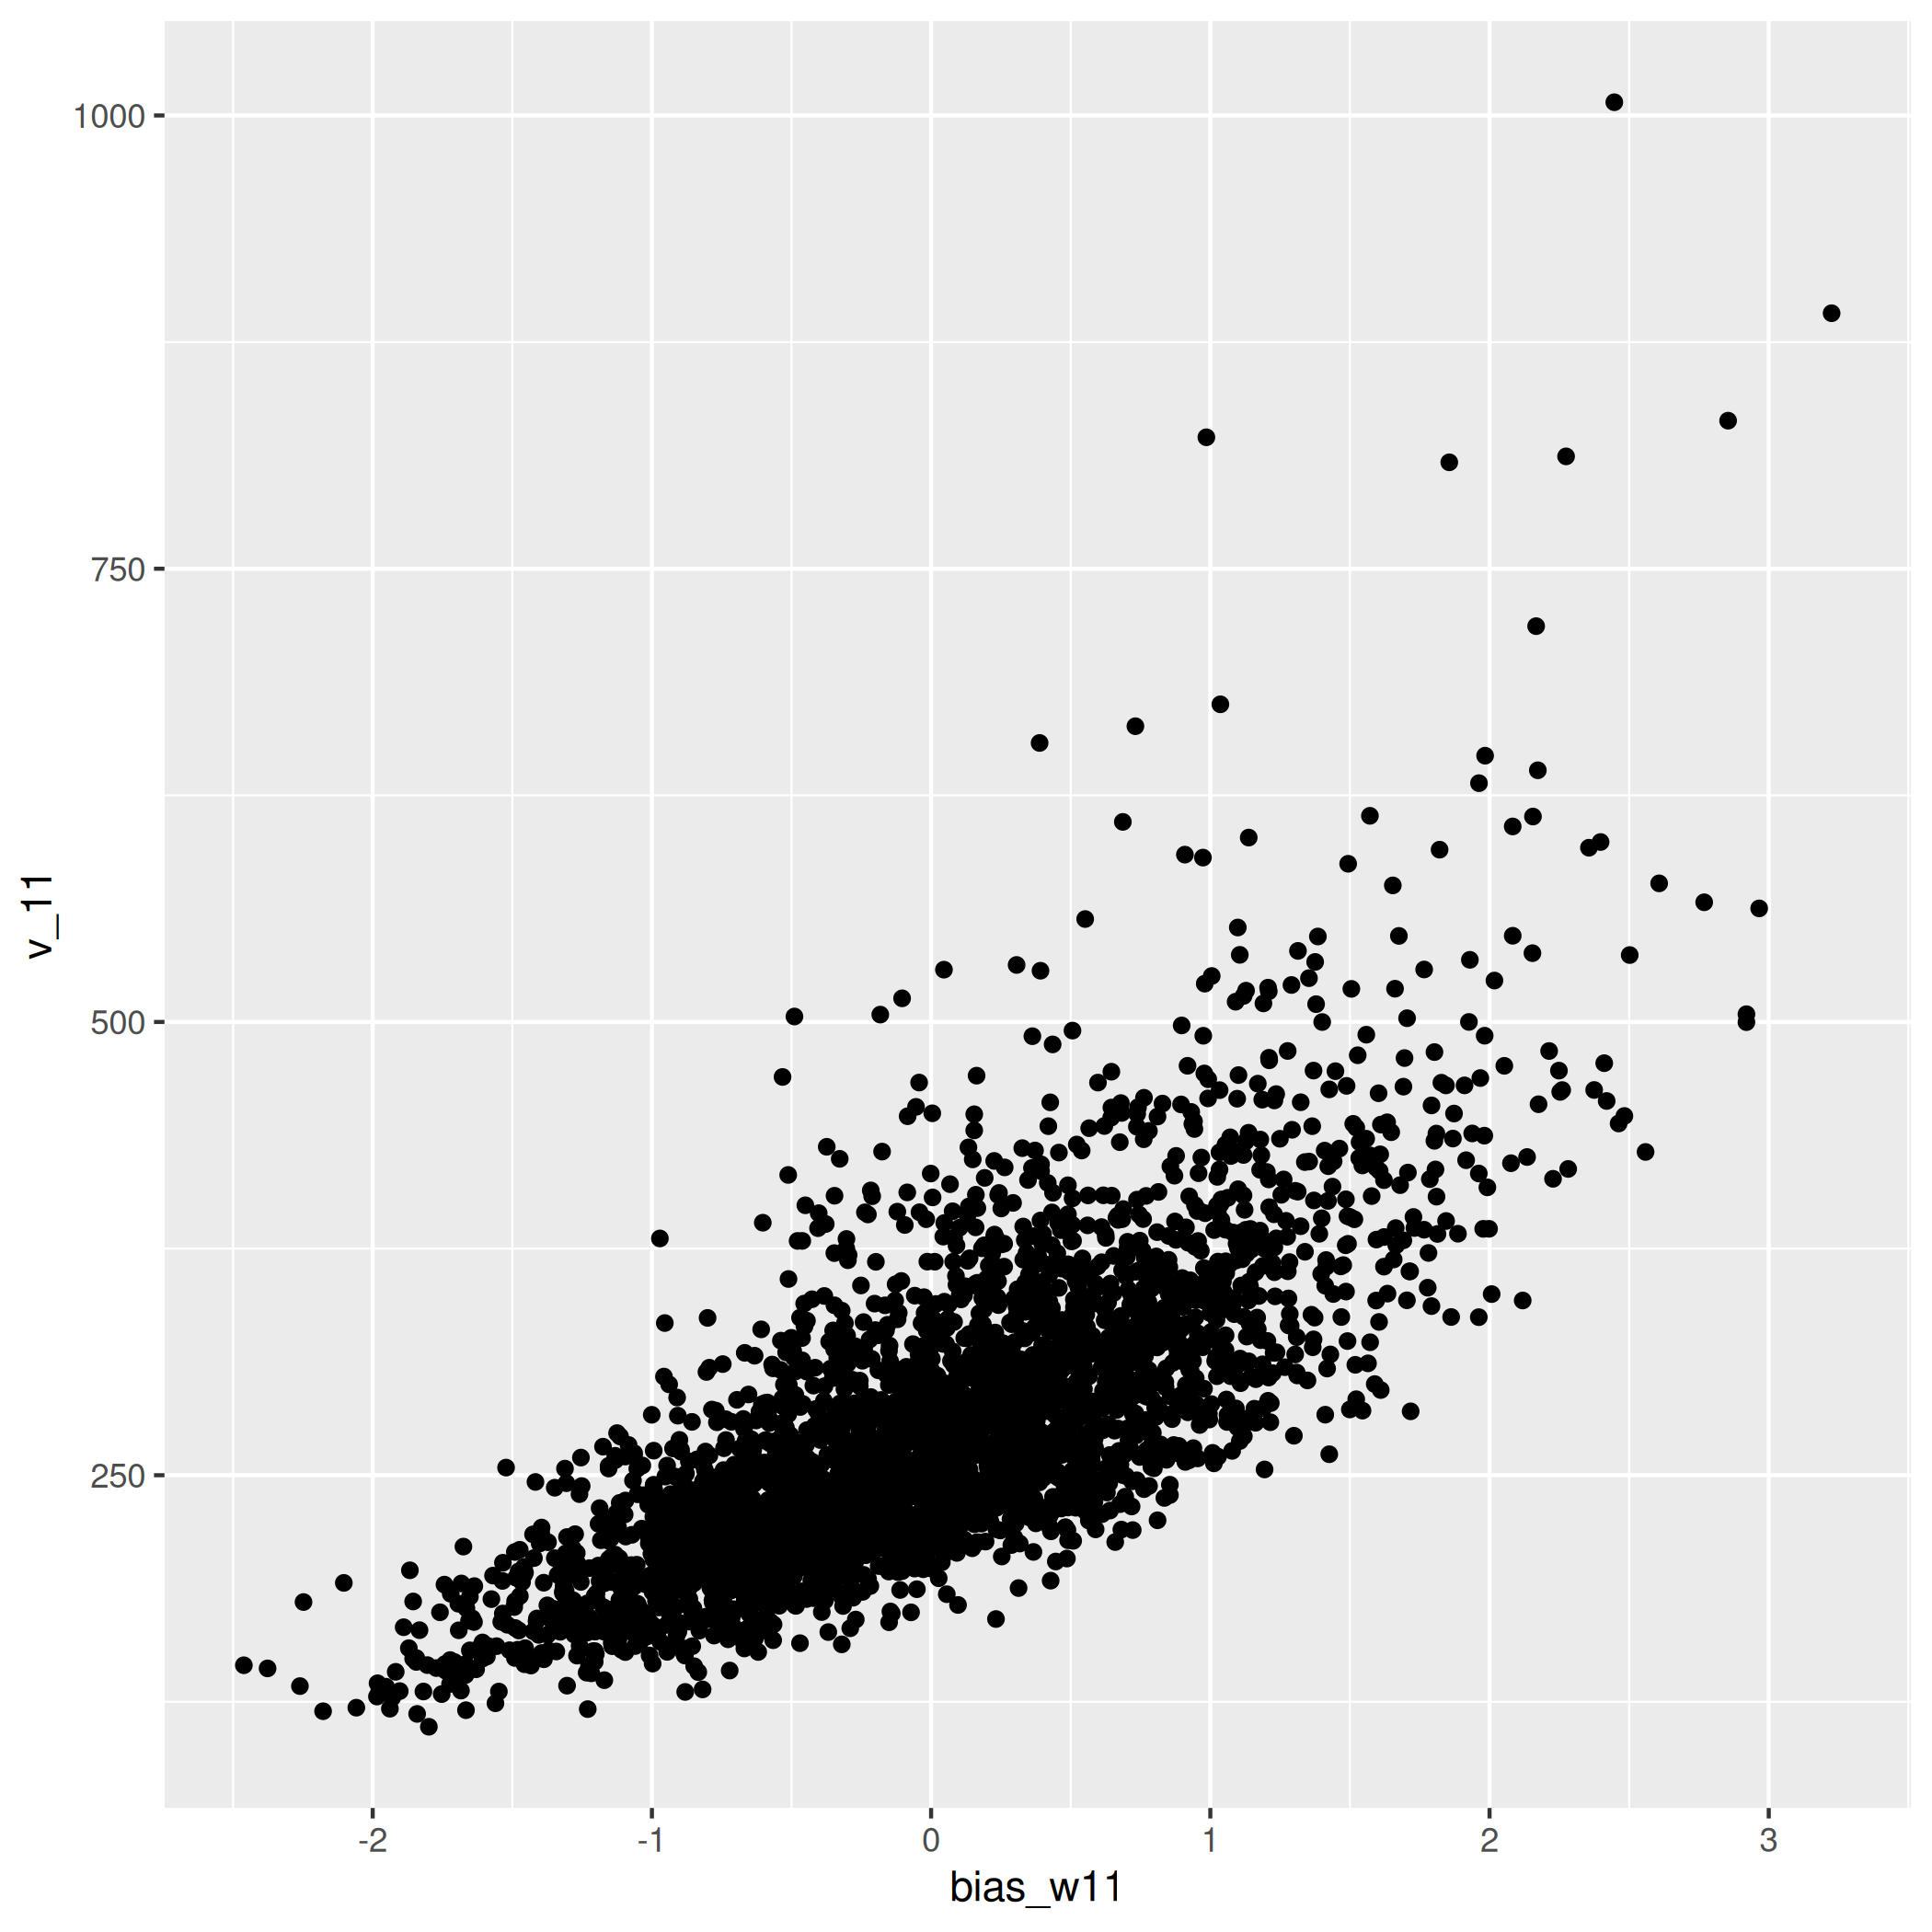
\includegraphics[width=7cm]{Images/biasvar_11.png}
\end{figure}

Figure~\ref{fig:biasvar} shows that the variance increases as the bias 
becomes more positive. This means that higher estimates will have 
a higher variance. Since we take the inverse variance weighted average 
of the four estimators, we are putting more weight on smaller estimators 
which will lead to a negative bias of our linear estimator which we 
observe in Table~\ref{tab:sim2}.

\end{document}
